\documentclass[a4paper,10pt]{article}
\usepackage[utf8x]{inputenc}
\usepackage{amsmath}
\usepackage{hyperref}
\usepackage{color}
\usepackage{subfigure}
\usepackage{graphicx}
\RequirePackage{algorithmic}


%opening
\title{Robot Localization Simulator}
\author{}


\newtheorem{theorem}{Theorem}
\newtheorem{lemma}[theorem]{Lemma}
\newtheorem{example}[theorem]{Example}
\newtheorem{remark}[theorem]{Remark}
\newtheorem{definition}[theorem]{Definition}
\newtheorem{proposition}[theorem]{Proposition}
\newtheorem{corollary}[theorem]{Corollary}



\begin{document}

\maketitle

\begin{abstract}
In this project we explore the various algorithms for the Robot Localization Problem and build a simulator to visualize the results on
various 2D maps.
Robot localization is an important problem in robotics. Simply put, the robot localization problem is as follows. A robot is 
placed at an unknown point inside a simple polygon $ P $. The robot has a map of 
$ P$ and can compute visibility polygon from its current location. The robot must determine its correct 
location inside the polygon $P $ at a minimum cost of travel distance. We implement an ${O(\log^3 n)} $ factor approximation algorithm 
as given by \cite{key1}. CGAL \cite{key2} has been used for the various computational geometry algorithms.

\end{abstract}

\newpage
\section{Robot Localization Algorithm}

{\bf Input:}\\
Map polygon $P$, the visibility polygon $V$.
\\
{\bf Output:}\\
The robot localizes to its actual position $h \in H$
\\
\begin{algorithmic}[1]
  \STATE Compute the set of hypotheses $H$.
 \WHILE{ $ | H | > 1$ } 
  \STATE Compute the majority-rule map $P_{maj}$
  \STATE Compute the polygons $G_{ij}$ for each pair of hypotheses, $h_{i}$ and $h_{j}$
  \STATE Compute the majority rule map $K_{i}$ of $G_{ij}$'s
  \STATE Find the edges on the boundary of $K_{i}$ which are not on the boundary of $P_{maj}$
  \STATE Draw grids and compute the set of coordinates $Q_{H}$ on these edges.
  \STATE Make instance $I_{P,H}$  of $\frac{1}{2}$ -Group Steiner Problem
  \STATE Solve $I_{P,H}$ to compute a half computing path $C \subset P_{maj}$
  \STATE Half-Localize by tracing $C $ and making observations at coordinates $Q_{H}$
  \STATE Move back to the starting location.
 \ENDWHILE
\end{algorithmic}

\newpage















\section{Notation}
\begin{itemize}
\item
{\bf $H$}: A list of points which denotes potential robot positions.


\item
{\bf $P_{maj}$}: The majority rule map of all translates of the polygon. The
translates of the polygon are obtained by choosing one hypothesis as the origin and
translating all the remaining hypotheses to this chosen origin.


\item
{\bf $G_{ij}$}: For the translates corresponding to pair of hypotheses $h_{i}$ and
 $h_{j}$, $G_{ij}$ is the origin containing region obtained by taking the lower
envelope of visibility polygons of all type 1 and type 2 edges of the polygon.\\
An edge is of type 1 or type 2, if it belongs to exactly one of the translates.

\item
{\bf $g_{i}$}: The set of all points at which $h_{i}$ does not share the majority
opinion about $i$.

\item
{\bf $K_{i}$}: The majority rule map of $G_{ij}$'s

\item
{\bf $Maj(\gamma)$}: Set of hypothesis which share the majority opinion about $\gamma$. $\gamma$ can be either a point
or a region.

\end{itemize}














\newpage

\section{Computing Visibility Polygons}
Visibility polygon is an indispensable component is the hypothesis generation step of the algorithm. Since CGAL had no inbuilt support
 for computing visibility polygons we implemented the following two routines for our purposes.
\begin{itemize}
 \item Visibility Polygon of a point inside a polygon
 \item Visibility Polygon of an edge of the polygon.
\end{itemize}

\subsection{Visibility Polygon of a Point Inside a Polygon}

The following is the C++ function in the file PolygonUtil.cpp. We pass the map polygon and the point $P$, whose visibility polygon is to be
 computed. The function returns the visibility polygon of $P$ as another Polygon type.
In $setVisiblePoints$ we collect all those points which are directly visible from $P$. Note that
 all these points will form a part of the visibility polygon of $P$ since they are directly visible from $P$. 
Besides these some additional spurious vertices will also be introduced. Each spurious vertex which is a part of the visibility polygon
 can be obtained by extending the line joining the point $P$ to some reflex vertex. We do this in the if block and collect all the 
spurious vertices also. Finally we sort all the vertices obtained in an order so that they form the visibility polygon of $P$.



{\bf Algorithm}

\begin{enumerate}
 \item 
Collect all the vertices of the polygon which are visible from the point $P$.
\item
Iterate over the list of visible vertices and for each reflex vertex, compute the spurious vertex introduced in the visibility polygon.
\item
Finally sort all the vertices in an order so that they form a simple polygon.
\end{enumerate}

{\bf Examples}

The point $P$ is shown in blue and the visibility polygon is shown in green.

\begin{figure}[h]
\begin{center}
\scalebox{0.30}{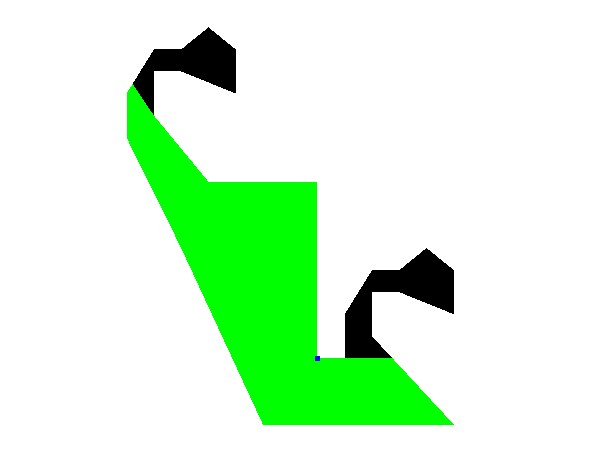
\includegraphics{Images/VisibilityPolygonBird.png}}
\caption{\label{fig:Visibility Polygon of Point}Visibility Polygon of Point}
\end{center}
\end{figure}


\begin{figure}[h]
\begin{center}
\scalebox{0.40}{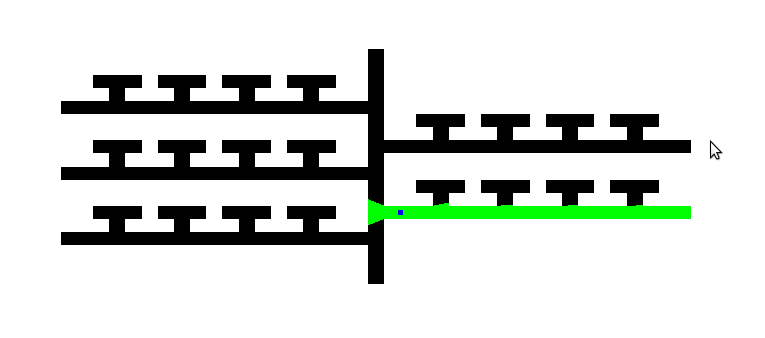
\includegraphics{Images/VisibilityPointOffice.png}}
\caption{\label{fig:Visibility Polygon of Point}Visibility Polygon of Point}
\end{center}
\end{figure}





%Java2TeX style definitions
%You can modify them to fit your needs
\newcommand{\jttstylea}{\color[rgb]{1.00,1.00,1.00}} %Background
\newcommand{\jttstyleb}{\color[rgb]{.501,.501,.501}} %Line numbers
\newcommand{\jttstylec}{\color[rgb]{.247,.498,.372}} %Multi-line comments
\newcommand{\jttstyled}{\color[rgb]{.247,.498,.372}} %Single-line comments
\newcommand{\jttstylee}{\color[rgb]{.498,.000,.333}} %Keywords
\newcommand{\jttstylef}{\color[rgb]{.164,.000,1.00}} %Strings
\newcommand{\jttstyleg}{\color[rgb]{.600,.000,.000}} %Character constants
\newcommand{\jttstyleh}{\color[rgb]{.600,.000,.000}} %Numeric constants
\newcommand{\jttstylei}{\color[rgb]{.000,.000,.000}} %Parenthesis
\newcommand{\jttstylej}{\color[rgb]{.498,.000,.333}} %Primitive Types
\newcommand{\jttstylek}{\color[rgb]{.000,.000,.000}} %Others
\newcommand{\jttstylel}{\color[rgb]{.498,.623,.749}} %Javadoc keywords
\newcommand{\jttstylem}{\color[rgb]{.498,.498,.623}} %Javadoc HTML tags
\newcommand{\jttstylen}{\color[rgb]{.247,.247,.749}} %Javadoc links
\newcommand{\jttstyleo}{\color[rgb]{.247,.372,.749}} %Javadoc others
\newcommand{\jttstylep}{\color[rgb]{1.00,.380,.000}} %Undefined
\newcommand{\jttstyleq}{\color[rgb]{.392,.392,.392}} %Annotation




\subsection{Visibility Polygon of an edge of the polygon}
The algorithm for the visibility polygon of an edge has been taken from \cite{key3}.
Let $E$ be the set of edges of the polygon. To find the visibility polygon of an edge $AB$, we compute, for each of 
 the remaining edges of the polygon the portion of it which is weakly visible from the edge $AB$. Once we obtain these portions we join
 all of them to obtain the visibility polygon of the edge $AB$.
  Implementation of this algorithm requires computing shortest path between vertices of the polygon, the construction of which we 
describe in the next section. For now assume that we have at our disposal a routine which gives the shortest path between two vertices 
of the polygon as a list of Point type.

The main steps of computing the visible portion of an edge $CD$ from another edge $AB$ of the polygon can be enumerated as follows.

{\bf Algorithm}



\begin{enumerate}
\item
Compute the shortest path $P_{AC}$, from A to C and the shortest path $P_{BD}$, from B to D. Call this pair 1.
\item
Similarly compute the shortest path  $P_{AD}$, from A to D and the shortest path  $P_{BC}$,  from B to C. Call this pair 2.
\item
Find out which of these pairs is outward convex. An outward convex pair implies an hourglass shape is formed by the two paths.
\item
If none of the pairs is outward convex this means that no portion of edge $CD$ is visible from any point on edge $AB$ and we can 
completely ignore such an edge.

\begin{figure}[h]
\begin{center}
\scalebox{0.50}{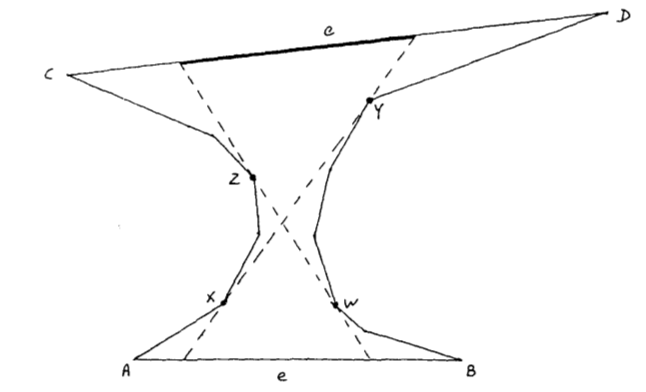
\includegraphics{Images/Cusp.png}}
\caption{\label{fig:Visibility Polygon of Edge}Visibility Polygon of Edge, Illustration taken from:\cite{key3}}
\end{center}
\end{figure}

\item
If one of the pairs is outward convex then without loss of generality, let pair 1 be the outward convex pair. Now compute the shortest 
paths  $P_{AD}$ and  $P_{BC}$.

\item
Let $X$ be the point where path $P_{AD}$ and $P_{AC}$ split and let  $W$ be the point where path $P_{BD}$ and $P_{BC}$ split. Let $Y$ be
the next point on the path  $P_{AD}$ and $Z$ be the next point on the path   $P_{BC}$. Extending $XY$ we get one extreme point of the 
portion of $CD$ visible from $AB$. We repeat this on other side to get the other extreme point.


\end{enumerate}

 $CalcVisibilityPolygonEdge()$ calculates the visibility polygon of an edge in PolygonUtil.cpp

{\bf Note:}
This routine computes the visibility polygon of the edge excluding its endpoints. To obtain the visibility polygon of the edge where
endpoints are inclusive one could compute the visibility polygon of point at the two endpoints and take a union with the visibility
polygon returned by this routine.

\begin{figure}[h]
\begin{center}
\scalebox{0.50}{
\includegraphics{Images/VisibilityLine1.png}}
\caption{\label{fig:Visibility Polygon of Edge}Visibility Polygon of Edge}
\end{center}
\end{figure}



\subsection{Shortest Path Calculation}
For the calculation of shortest path between any two vertices of the polygon the following property was exploited.
\begin{itemize}
 \item The shortest path must turn only at vertices of the polygon.
 \item It is possible to move from one vertex to the another only if they are visible to each other.
\end{itemize}

\begin{definition}
{\bf Visibility Graph}The visibility graph of a polygon can be formed as follows. Draw a vertex corresponding to each vertex in the 
polygon. Draw an edge between two vertices if the line joining the corresponding vertices in the polygon lies completely inside the 
polygon.
\end{definition}


Utilizing these properties we construct a visibility graph for the polygon and use the normal dijikstra's single source shortest path
 algorithm on the visibility graph obtained. The following two functions do the above mentioned tasks.



\begin{itemize}


\item
%Java2TeX style definitions
%You can modify them to fit your needs

%%%%%%%%%%%%%%%%%%%%%%%%%%%%%%%%%%%%%%%%%%%%%%%%%%%%%%%%%%%%%%%
%  Java Sourcecode to TeX automatically converted code
%  Java2Html Converter 5.0 [2006-02-26]by Markus Gebhard  markus@jave.de
%     Further information: http://www.java2html.de
{
\noindent \ttfamily
\noindent \ttfamily
\noindent \ttfamily
\noindent \ttfamily
\jttstylek PolygonUtil::PrepareVisibilityGraph\jttstylei (\jttstylek Polygon\&~map,~Point~vertex\jttstylei [])\\

}


\item
%Java2TeX style definitions
%You can modify them to fit your needs

%%%%%%%%%%%%%%%%%%%%%%%%%%%%%%%%%%%%%%%%%%%%%%%%%%%%%%%%%%%%%%%
%  Java Sourcecode to TeX automatically converted code
%  Java2Html Converter 5.0 [2006-02-26]by Markus Gebhard  markus@jave.de
%     Further information: http://www.java2html.de
{
\noindent \ttfamily
\jttstylek PolygonUtil::CalcShortestPath\jttstylei (\jttstylej int~\jttstylek source,graph\verb#_#t\&~g,Point~vertex\jttstylei [])\\
\noindent \ttfamily
}

\end{itemize}

{\bf Examples}

The edge is shown in blue and its visibility polygon is shown in green.

\begin{figure}[h]
\begin{center}
\scalebox{0.40}{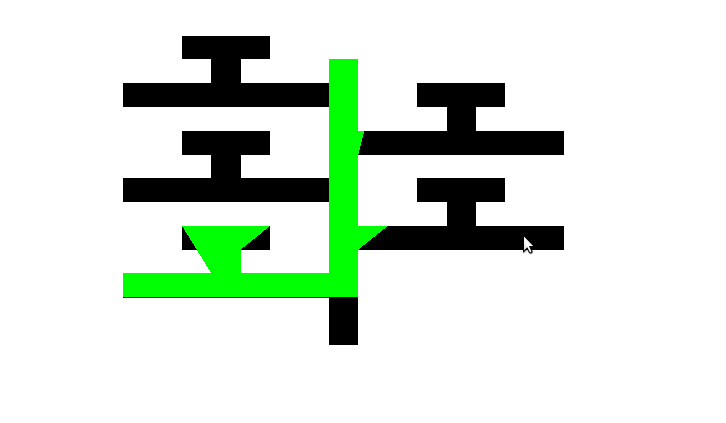
\includegraphics{Images/VisibilityLine2.png}}
\caption{\label{fig:Visibility Polygon of Edge}Visibility Polygon of Edge}
\end{center}
\end{figure}


















\newpage
\section{Hypothesis Generation}
Hypothesis Generation phase is based on the following conjecture which we try to prove in the next subsection.

\begin{theorem}
 A point, $P$ inside a simple polygon sees atleast one edge of the polygon completely.
\end{theorem}
The proof of the above theorem comes from the following two simple facts.
\begin{itemize}
 \item An edge is partially visible from a point inside the polygon only if it is occluded partially by another reflex vertex of the polygon
not belonging to that edge.
\item A reflex vertex can occlude one and only one edge of the polygon.
\end{itemize}

To prove the theorem for any arbitrary polygon we obtain the visibility polygon of point P and show that atleast one edge of this
visibility polygon, which is also an edge of the original polygon, is completely visible from point $P$. Alternatively Theorem 1 can be
 restated as follows.

\begin{definition}
 {\bf Spurious Edge:} In the visibility polygon of a point, an edge is called a spurious edge if it is obtained by extending the line
 joining the point $P$ and a reflex vertex till it meets the polygon.
\end{definition}


\begin{theorem}
 The visibility polygon of a point $P$ has atleast one edge which completely overlaps with an edge of the original polygon.
\end{theorem}
{\bf Proof} Let the visibility polygon be $V$. Let the visibility polygon have $n$ non-spurious edges and $r$ spurious edges.
Each of the spurious edge is due to a reflex vertex, so the polygon would have $r$ reflex vertices at least.
 According to the theorem, one of the $n$ edges must overlap completely with an edge of the polygon.
We prove it by contradiction. Assume to the contrary that all of the $n$ edges are partially visible from $P$. Thus each of the $n$
edges must be occluded by a reflex vertex $v$ not lying on the edge. And since a reflex vertex cannot occlude multiple edges, therefore
 a total of $n$ reflex vertices will be required to occlude the $n$ edges.
So such a polygon, if it exists, should have $n+r$ reflex vertices, but it is not possible to construct a closed polygon with all
 vertices as reflex vertex.
Hence our original assumption was wrong.

{\bf Algorithm}

\begin{enumerate}
 \item Iterate over the edges of the polygon and the edges of the map. and find an edge in the map which has the same length and
 orientation as an edge in the polygon.

 \item
 Translate the visibility polygon such that the matching edge of the map polygon
and the visibility polygon coincide.

 \item
 For each of the remaining edges of the visibility polygon, check whether a 
complete match exists or not. If all the remaining edges match, the point where the
origin was translated is added to the set of hypotheses.

\end{enumerate}

\newpage

{\bf Examples}

\begin{figure}[h]
\begin{center}
\scalebox{0.40}{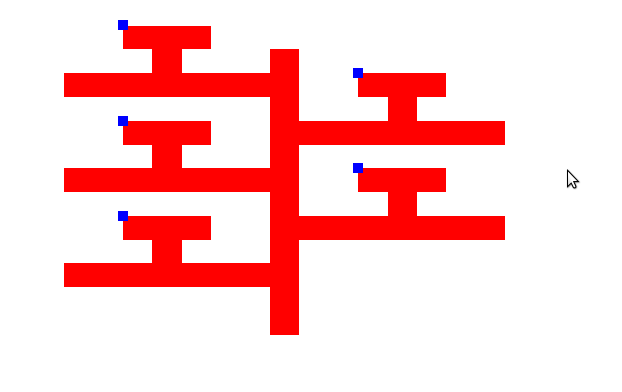
\includegraphics{Images/Hypothesis_office.png}}
\caption{\label{fig:Hypothesis Generation}Hypothesis Generation}
\end{center}
\end{figure}


\begin{figure}[h]
\begin{center}
\scalebox{0.40}{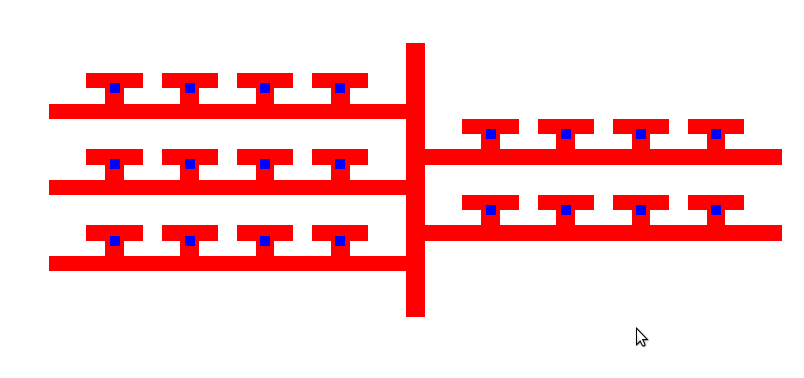
\includegraphics{Images/HypothesisOfficeAnti.png}}
\caption{\label{fig:Hypothesis Generation}Hypothesis Generation}
\end{center}
\end{figure}

















\newpage

\section{Computing the Majority Rule Map $P_{maj}$}

\subsection{Construction}
The following example taken from \cite{key1} demonstrates the construction of a majority rule map.

\begin{figure}[h]
\begin{center}
\scalebox{0.50}{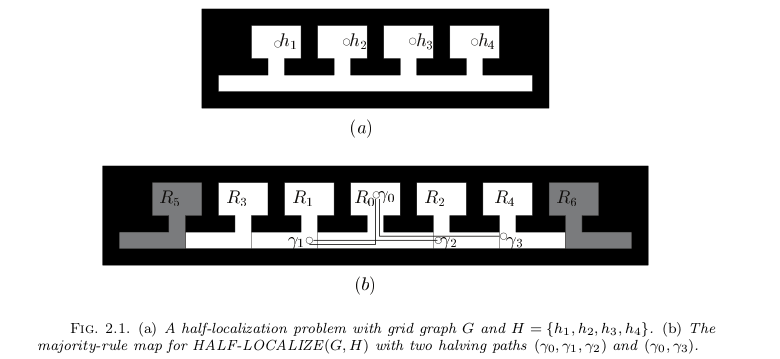
\includegraphics{Images/MajorityMapExample.png}}
\caption{\label{fig:Construction}Majority Rule Map Construction}
\end{center}
\end{figure}

${h_{1},h_{2},h_{3},h_{4}}$ form the set of hypotheses. Arbitrarily we choose $h_{1}$ as the origin. Next we translate all the 
remaining hypotheses to $h_{1}$ to obtain the overlay arrangement. The overlay arrangement contains the following faces
$R_{0},R_{1},R_{2},R_{3},R_{4},R_{5},R_{6}$. Recall from the definition of $Maj(\gamma)$



$  Maj(R_{0})  =  {h_{1}, h_{2}, h_{3}, h_{4}} $ , $  Maj(R_{1})  =  { h_{2}, h_{3}, h_{4}} $, $ Maj(R_{2})  =  {h_{1}, h_{2}, h_{3}} $,
$  Maj(R_{3})  =  {h_{3}, h_{4}} $ and $  Maj(R_{4})  =  {h_{1}, h_{2}} $



In the majority rule map the region $R_{5}$ and $R_{6}$ are blocked because less than half the hypothesis said that they were
 traversable. They have been shown in gray.

\begin{figure}[h]
\begin{center}
\scalebox{0.40}{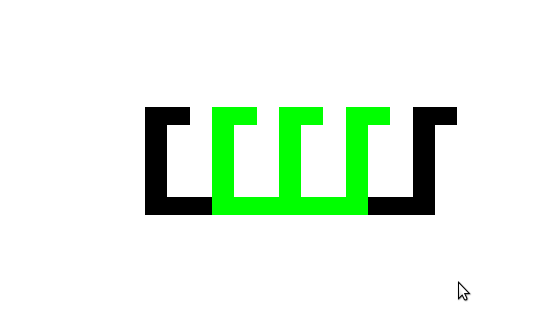
\includegraphics{Images/MajorityMapScenario1.png}}
\caption{\label{fig:Majority Rule Map}Majority Rule Map shown in green}
\end{center}
\end{figure}





\newpage
\subsection{Majority Rule Map Type}

The Majority Rule Map is represented as a class. The following code demonstrates the values stored along with a majority rule map and the 
functions applicable on it.




%%%%%%%%%%%%%%%%%%%%%%%%%%%%%%%%%%%%%%%%%%%%%%%%%%%%%%%%%%%%%%%
%  Java Sourcecode to TeX automatically converted code
%  Java2Html Converter 5.0 [2006-02-26]by Markus Gebhard  markus@jave.de
%     Further information: http://www.java2html.de
{
\noindent \ttfamily
\jttstylea \\
\jttstylea \\
\jttstylea \\
\jttstylea \\
\jttstylee class~\jttstylek Majoritymap~\jttstylei \{\\
\jttstylee public\jttstylek :\\
\jttstylea \\
\jttstylea ~~\jttstylek list\verb#<#Faces\verb#>#~listMmapFaces;\\
\jttstylea ~~\jttstylek Polygon~map;\\
\jttstylea ~~\jttstylej int~\jttstylek noOfHypothesis;\\
\jttstylea ~~\jttstylek Point~\verb#*#hypothesis;\\
\jttstylea ~~\jttstylek Point~center;\\
\jttstylea ~~\jttstylek list\verb#<#Polygon\verb#>#~listTanslatedPolygons;\\
\jttstylea ~~\jttstylek Arrangement~mmapArrangement;\\
\jttstylea \\
\jttstylea ~~\jttstylek PolygonUtil~pUtil;~\jttstyled //For~using~polygon~util~functions.\\
\jttstylea \\
\jttstylea ~~\jttstylek Majoritymap\jttstylei ()\jttstylek ;\\
\jttstylea ~~\jttstylek Majoritymap\jttstylei (\jttstylej int~\jttstylek n,~Point~H\jttstylei []\jttstylek ,Point~c,Polygon~P\jttstylei )\jttstylek ;\\
\jttstylea ~~\jttstylek Majoritymap\jttstylei (\jttstylej int~\jttstylek n,std::list\verb#<#Polygon\verb#>#~PolygonList\jttstylei )\jttstylek ;\\
\jttstylea \\
\jttstylea \\
\jttstylea ~~\jttstylej void~\jttstylek PrintMajorityMap\jttstylei ()\jttstylek ;\\
\jttstylea ~~\jttstylej void~\jttstylek GenerateMajorityMap\jttstylei ()\jttstylek ;\\
\jttstylea ~~\jttstylek Polygon~GetTranslatePolygon\jttstylei (\jttstylek Transformation\&~translate,~Polygon\&~polygon\jttstylei )\jttstylek ;\\
\jttstylea ~~\jttstylek Polygon~ConvertFaceToPolygon\jttstylei (\jttstylek Arrangement::Ccb\verb#_#halfedge\verb#_#const\verb#_#circulator~circ\jttstylei )\jttstylek ;\\
\jttstylea ~~\jttstylek bool~IsContainedIn\jttstylei (\jttstylek Polygon~outer,Polygon~inner\jttstylei )\jttstylek ;\\
\jttstylea ~~\jttstylek bool~CheckPartOfMajorityMap\jttstylei (\jttstylej int~\jttstylek agree,~\jttstylej int~\jttstylek noOfHypothesis\jttstylei )\jttstylek ;\\
\jttstylea \\
\jttstylea ~~\jttstylek list\verb#<#Polygon\verb#>#~findRegionContaningOrigin\jttstylei ()\jttstylek ;\\
\jttstylea ~~\jttstylek bool~areAdjacent\jttstylei (\jttstylek Polygon\&~poly1,~Polygon\&~poly2\jttstylei )\jttstylek ;\\
\jttstylea \\
\jttstylea ~~\jttstylek Polygon~OverlayContaningOrigin\jttstylei (\jttstylek Point~\&center\jttstylei )\jttstylek ;\\
\jttstylea \\
\jttstylea ~~\jttstylej void~\jttstylek GenerateOverlay\jttstylei (\jttstylek list\verb#<#Polygon\verb#>#~polygonList\jttstylei )\jttstylek ;\\
\jttstylea ~~\jttstylej void~\jttstylek partMajority\jttstylei ()\jttstylek ;\\
\jttstylea ~~\jttstylek virtual~\verb#~#Majoritymap\jttstylei ()\jttstylek ;\\
\jttstylei \}\jttstylek ;\\
\jttstylea \\
\jttstylea \\
\jttstylea \\
\jttstylea \jttstylea 
\\

}

Each majority rule map is basically a collection of faces. Faces is another type that encapsulates information about the opinion of 
each of the hypotheses about that face. Here is the Faces class.

%%%%%%%%%%%%%%%%%%%%%%%%%%%%%%%%%%%%%%%%%%%%%%%%%%%%%%%%%%%%%%%
%  Java Sourcecode to TeX automatically converted code
%  Java2Html Converter 5.0 [2006-02-26]by Markus Gebhard  markus@jave.de
%     Further information: http://www.java2html.de
{
\noindent \ttfamily
\jttstylea \\
\jttstylee class~\jttstylek Faces~\jttstylei \{\\
\jttstylee public\jttstylek :\\
\jttstylea ~~\jttstylek Polygon~face;\\
\jttstylea ~~\jttstylej int~\jttstylek noOfHypothesis;\\
\jttstylea ~~\jttstylek bool~\verb#*#containedIn;\\
\jttstylea ~~\jttstylek bool~partOfMajorityMap;\\
\jttstylea ~~\jttstylek Faces\jttstylei ()\jttstylek ;\\
\jttstylea ~~\jttstylek Faces\jttstylei (\jttstylej int~\jttstylek n,Polygon~p,~bool~\verb#*#A,bool~partMmap\jttstylei )\jttstylek ;\\
\jttstylea ~~\jttstylek Faces\jttstylei (\jttstylek Polygon~p\jttstylei )\jttstylek ;\\
\jttstylea ~~\jttstylej void~\jttstylek PrintDescription\jttstylei ()\jttstylek ;\\
\jttstylea ~~\jttstylek virtual~\verb#~#Faces\jttstylei ()\jttstylek ;\\
\jttstylei \}\jttstylek ;\\

}

Each Face has a bool flag partOfMajorityMap, which is true if this face is a part of the majority map i.e. atleast half of the 
hypotheses say that this face is traversable and false otherwise. It also has an bool array to specifically store the opinion of
 each of the hypothesis about this face.

\newpage
\subsection {CGAL's Arrangement class to generate Overlay}



%Java2TeX style definitions
%You can modify them to fit your needs

%%%%%%%%%%%%%%%%%%%%%%%%%%%%%%%%%%%%%%%%%%%%%%%%%%%%%%%%%%%%%%%
%  Java Sourcecode to TeX automatically converted code
%  Java2Html Converter 5.0 [2006-02-26]by Markus Gebhard  markus@jave.de
%     Further information: http://www.java2html.de
{
\noindent \ttfamily
\jttstylea \\
\jttstylea \\
\jttstylea \\
\jttstylej void~\jttstylek Majoritymap::GenerateOverlay\jttstylei (\jttstylek list\verb#<#Polygon\verb#>#~polygonList\jttstylei )\\
\jttstylei \{\\
\jttstylea \\
\jttstylea ~~\jttstylek list\verb#<#Polygon\verb#>#::iterator~pi;\\
\jttstylea \\
\jttstylea ~~\jttstylee for\jttstylei (\jttstylek pi=polygonList.begin\jttstylei ()\jttstylek ;pi!=polygonList.end\jttstylei ()\jttstylek ;++pi\jttstylei )\\
\jttstylea ~~\jttstylei \{\\
\jttstylea ~~~~\jttstylee for~\jttstylei (\jttstylek EdgeIterator~ei~=~pi-\verb#>#edges\verb#_#begin\jttstylei ()\jttstylek ;~ei~!=~pi-\verb#>#edges\verb#_#end\jttstylei ()\jttstylek ;~++ei\jttstylei )\\
\jttstylea ~~~~\jttstylei \{\\
\jttstylea ~~~~~~\jttstylek Point~s=ei-\verb#>#start\jttstylei ()\jttstylek ;\\
\jttstylea ~~~~~~\jttstylek Point~d=ei-\verb#>#end\jttstylei ()\jttstylek ;\\
\jttstylea ~~~~~~\jttstylek Point\verb#_#2~source\jttstylei (\jttstylek s.cartesian\jttstylei (\jttstyleh 0\jttstylei )\jttstylek ,s.cartesian\jttstylei (\jttstyleh 1\jttstylei ))\jttstylek ;\\
\jttstylea ~~~~~~\jttstylek Point\verb#_#2~destination\jttstylei (\jttstylek d.cartesian\jttstylei (\jttstyleh 0\jttstylei )\jttstylek ,d.cartesian\jttstylei (\jttstyleh 1\jttstylei ))\jttstylek ;\\
\jttstylea ~~~~~~\jttstylek Segment\verb#_#2~seg\jttstylei (\jttstylek source,~destination\jttstylei )\jttstylek ;\\
\jttstylea ~~~~~~\jttstylek CGAL::insert~\jttstylei (\jttstylek mmapArrangement,seg\jttstylei )\jttstylek ;\\
\jttstylea ~~~~\jttstylei \}\\
\jttstylea ~~\jttstylei \}\\
\jttstylea \\
\jttstylea \\
\jttstylea ~~\jttstylek Arrangement::Face\verb#_#const\verb#_#iterator~fit;\\
\jttstylea \\
\jttstylea ~~\jttstylee for~\jttstylei (\jttstylek fit~=~mmapArrangement.faces\verb#_#begin\jttstylei ()\jttstylek ;~fit~!=~mmapArrangement.faces\verb#_#end\jttstylei ()\jttstylek ;~++fit\jttstylei )\\
\jttstylea ~~\jttstylei \{\\
\jttstylea ~~~~\jttstylee if~\jttstylei (\jttstylek !fit-\verb#>#is\verb#_#unbounded\jttstylei ())\\
\jttstylea ~~~~\jttstylei \{\\
\jttstylea ~~~~~~\jttstylek Polygon~p=ConvertFaceToPolygon\jttstylei (\jttstylek fit-\verb#>#outer\verb#_#ccb\jttstylei ())\jttstylek ;\\
\jttstylea ~~~~~~\jttstylek Faces~f\jttstylei (\jttstylek p\jttstylei )\jttstylek ;\\
\jttstylea ~~~~~~\jttstyled //constructing~the~overlay~Arrangement~by~adding~the~faces~as~polygons.\\
\jttstylea ~~~~~~\jttstylek listMmapFaces.push\verb#_#back\jttstylei (\jttstylek f\jttstylei )\jttstylek ;\\
\jttstylea ~~~~\jttstylei \}\\
\jttstylea \\
\jttstylea ~~\jttstylei \}\\
\jttstylei \}\\
\jttstylea \\
\jttstylea \jttstylea 
\\

}
First we insert all edges in the region using CGAL::insert (mmapArrangement,seg). The Arrangement class which is inbuilt in CGAL 
automatically generates all faces that can be formed by the intersection of the edges.


\newpage


\subsection{Algorithm}
\begin{enumerate}
\item
The overlay arrangement can be easily constructed using CGAL's inbuilt Arrangement class. Obtain the translates of the polygon by 
choosing one hypothesis as the origin and shifting other hypothesis to it.
\item
Insert all these translates in CGAL's inbuilt arrangement to obtain all the faces in the overlay arrangement.
\item
Faces which belong to atleast half the hypothesis are marked as part of the majority rule map.
\end{enumerate}


{\bf Examples}


\begin{figure}[h]
\begin{center}
\scalebox{0.50}{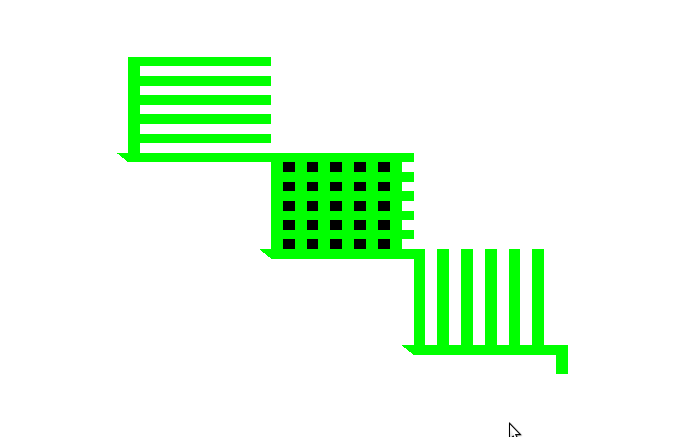
\includegraphics{Images/MajorityMapScenario4.png}}
\caption{\label{fig:Majority Rule Map}Majority Rule Map}
\end{center}
\end{figure}











\newpage
\section{Computing $G_{ij}$'s}





\newpage

\begin{thebibliography}{1}
\bibitem{key1} \emph{A Near-Tight approximation algorithm for the robot localization problem},
 Koenig, Sven and Mudgal, Proceedings of the Symposium on Discrete Algorithms SODA, 2006.

\bibitem{key2} $<$\url{http://www.cgal.org/}$>$

\bibitem{key3} \emph{Linear time algorithms for visibility and shortest path problems inside simple polygons}, Guibas, 
Hershberger, Daniel Leven, Micha Sharir, Robert E. Tarjan
\end{thebibliography}







\end{document}
